%%
%% hibari_tda.tex — Topological Data Analysis of Ryuichi Sakamoto's "hibari"
%% IEEEtran class. Compile with pdflatex or xelatex (xelatex recommended for
%% Korean / Unicode support via fontspec).
%%
%% To compile (xelatex recommended):
%%   xelatex hibari_tda.tex
%%   bibtex hibari_tda     (optional, if adding .bib)
%%   xelatex hibari_tda
%%   xelatex hibari_tda
%%

\documentclass[conference,10pt,a4paper]{IEEEtran}

% ── Packages ─────────────────────────────────────────────────────────────
\usepackage[utf8]{inputenc}
\usepackage[T1]{fontenc}
\usepackage{amsmath, amssymb, amsthm}
\usepackage{graphicx}
\usepackage{booktabs}
\usepackage{multirow}
\usepackage{url}
\usepackage{cite}
\usepackage{algorithm}
\usepackage{algpseudocode}
\usepackage[hidelinks]{hyperref}
\usepackage{color}
\usepackage{xcolor}
\usepackage{enumitem}

% For Korean support when using xelatex, uncomment:
% \usepackage{fontspec}
% \usepackage{xeCJK}
% \setCJKmainfont{NanumGothic}

% ── Theorem environments ─────────────────────────────────────────────────
\newtheorem{definition}{Definition}
\newtheorem{theorem}{Theorem}
\newtheorem{remark}{Remark}

% ── Paths ────────────────────────────────────────────────────────────────
\graphicspath{{../figures/}}

% ── Title ────────────────────────────────────────────────────────────────
\title{Topological Data Analysis of Ryuichi Sakamoto's \emph{hibari}:\\
       A Persistent Homology Pipeline for Structure-Preserving Music Generation}

\author{\IEEEauthorblockN{Minju Kim}
\IEEEauthorblockA{Department of Mathematics\\
POSTECH (Pohang University of Science and Technology)\\
Pohang, Republic of Korea}
}

\begin{document}

\maketitle

% ═══════════════════════════════════════════════════════════════════════════
% ABSTRACT
% ═══════════════════════════════════════════════════════════════════════════
\begin{abstract}
We present a computational pipeline that extracts the topological structure
of a musical composition via persistent homology and re-synthesizes new
musical pieces that preserve that structure.  Applied to Ryuichi Sakamoto's
\emph{hibari} (from the 2009 album \emph{out of noise}), the pipeline
(i)~constructs a weighted note-network from the MIDI quantization,
(ii)~computes $H_1$ persistent homology under four distance functions
(frequency, Tonnetz, voice-leading, DFT),
(iii)~builds an overlap matrix recording cycle activations across the
timeline, and (iv)~generates new music via either probabilistic sampling
(Algorithm~1) or deep learning (Algorithm~2; FC / LSTM / Transformer).

Over $N=20$ independent trials, the Tonnetz distance reduces pitch
Jensen--Shannon divergence from $0.0753 \pm 0.0033$ (frequency baseline)
to $0.0398 \pm 0.0031$, a $47\%$ improvement (Welch $t = 35.1$,
$p < 10^{-20}$, Cohen's $d = 11.1$).  Continuous overlap with per-cycle
thresholding adds a further $47.5\%$ gain ($p < 0.001$), and soft
activation input to the FC model achieves JS~$= 0.0004$, less than
$0.1\%$ of the theoretical maximum~$\ln 2$.  The simplest FC model
outperforms LSTM and Transformer on \emph{hibari}, while this ranking
reverses on the chromatic \emph{solari}---confirming that a composition's
aesthetic character determines the optimal model architecture.

We further extend the pipeline to topology-preserving \emph{variation}:
note redistribution under Tonnetz matching constraints (DTW $+61.4\%$),
temporal reordering, and harmonic constraints, producing music that is
topologically similar yet melodically distinct from the original.
\end{abstract}

\begin{IEEEkeywords}
Persistent homology, Topological data analysis, Music generation,
Tonnetz, Jensen--Shannon divergence, Multi-label classification,
Vietoris--Rips complex, Overlap matrix.
\end{IEEEkeywords}

% ═══════════════════════════════════════════════════════════════════════════
% SECTION 1: INTRODUCTION
% ═══════════════════════════════════════════════════════════════════════════
\section{Introduction}
\label{sec:intro}

Topological Data Analysis (TDA) offers a principled way to extract
geometric structure from data that is robust to noise and to
uniform rescaling of the metric
\cite{carlsson2009,edelsbrunner2010}.  In this work, we apply TDA to
a specific musical composition---Ryuichi Sakamoto's \emph{hibari}---and
ask whether the topological invariants (specifically, the first
persistent homology group $H_1$) can serve as a structural seed for
generating new, stylistically faithful music.

\subsection{Research Questions}
\begin{enumerate}
\item How can the topological structure of music be defined
      mathematically via Vietoris--Rips $H_1$ persistence?
\item Can new music be generated that \emph{preserves} this structure,
      and how do we measure preservation quantitatively?
\item Does the choice of distance function (frequency, Tonnetz,
      voice-leading, DFT) significantly affect generation quality?
\end{enumerate}

\subsection{Why \emph{hibari}?}
\emph{hibari} is drawn from Sakamoto's experimental album
\emph{out of noise} (2009).  It offers:
(i)~adequate scale ($T = 1{,}088$ eighth-note timepoints, $N = 23$
distinct notes, $C = 17$ chords);
(ii)~a balance of simplicity (7 pitch classes, C major) and complexity
(two instruments with coprime period structure, \S\ref{subsec:phase});
(iii)~an aesthetic that privileges spatial note placement over temporal
causality, directly relevant to our model-selection findings (\S\ref{subsec:dl}).

\subsection{Contributions}
\begin{enumerate}
\item A four-stage pipeline (preprocessing $\to$ PH $\to$ overlap matrix
      $\to$ generation) with two generators and four distance functions.
\item Systematic $N=20$ statistical comparisons establishing Tonnetz as
      optimal for diatonic compositions.
\item Continuous overlap matrices with per-cycle thresholds
      (\S\ref{subsec:percycle}), yielding an additional $47.5\%$ JS gain.
\item Topology-preserving musical variation via Tonnetz-matching note
      redistribution, temporal reordering, and harmonic constraints
      (\S\ref{sec:extensions}).
\item Cross-composition validation on \emph{solari}, Bach, and Ravel,
      confirming that the composition's character determines the optimal
      distance function and model architecture (\S\ref{subsec:generalization}).
\end{enumerate}


% ═══════════════════════════════════════════════════════════════════════════
% SECTION 2: MATHEMATICAL BACKGROUND
% ═══════════════════════════════════════════════════════════════════════════
\section{Mathematical Background}
\label{sec:background}

\subsection{Vietoris--Rips Complex}
\label{subsec:vr}

\begin{definition}
Given a finite metric space $(X, d)$ and $\varepsilon > 0$, the
\emph{Vietoris--Rips complex} $\mathrm{VR}_\varepsilon(X)$ is the
simplicial complex
$\mathrm{VR}_\varepsilon(X) = \{\sigma \subseteq X \mid
\forall x_i, x_j \in \sigma,\; d(x_i,x_j) \le \varepsilon\}$.
\end{definition}

As $\varepsilon$ increases, the nested family
$\mathrm{VR}_0 \subseteq \mathrm{VR}_{\varepsilon_1} \subseteq \cdots$
forms a \emph{filtration}.  In this paper, $X$ consists of the 23
distinct notes of \emph{hibari}.

\subsection{Persistent Homology}
\label{subsec:ph}

The $n$-th homology group $H_n(K) = \ker\partial_n / \mathrm{im}\,\partial_{n+1}$ captures $n$-dimensional ``holes.''
We focus on $H_1$, whose generators correspond to topological cycles.
\emph{Persistent homology} tracks each cycle's birth~$b$ and death~$d$
across the filtration; $\mathrm{pers} = d - b$ measures stability.
Cycles with large persistence represent robust structural features.

We primarily use the pHcol algorithm from prior work
\cite{tran2021,lee2024} with cycle representatives, supplemented
by Ripser \cite{bauer2021} for speed-critical steps.

\subsection{Musical Distance Functions}
\label{subsec:distances}

We compare four distance functions between notes $n_i = (p_i, d_i)$:

\paragraph{Frequency distance (baseline)}
$d_{\mathrm{freq}}(n_i, n_j) = 1/w(n_i, n_j)$, where $w$ is
the adjacency frequency in the chord sequence.

\paragraph{Tonnetz distance}
Pitch classes are embedded on a hexagonal lattice with edges at
$\pm 3, \pm 4, \pm 7$ semitones (minor~3rd, major~3rd, perfect~5th).
The distance is the shortest graph path, pre-computed into a
$12 \times 12$ table (range $0$--$4$) \cite{tymoczko2012}.

\paragraph{Voice-leading distance}
$d_V(p_1, p_2) = |p_1 - p_2|$, the unsigned semitone difference
\cite{tymoczko2008}.

\paragraph{DFT distance}
Each pitch class $p$ is encoded as a 12-dimensional indicator vector
$\mathbf{e}_p \in \{0,1\}^{12}$.  Its discrete Fourier transform yields
magnitude coefficients $|F_k|$ for $k = 0, \ldots, 5$ (the first six
components suffice by symmetry).  The DFT distance is then the $L_2$
distance between these magnitude vectors:
$d_{\mathrm{DFT}}(p_1,p_2) = \sqrt{\sum_{k=0}^{5}(|F_k(p_1)| - |F_k(p_2)|)^2}$.
The maximum value is $\sqrt{2}$ (attained by maximally dissimilar
pitch classes such as C vs.\ F$\sharp$) \cite{tymoczko2008}.

\paragraph{Hybrid distance and note-level extensions}
All music-theoretic distances are combined with frequency via
$d_{\mathrm{hybrid}} = \alpha\, d_{\mathrm{freq}} + (1-\alpha)\, d_{\mathrm{music}}$,
where $\alpha \in [0,1]$.  Each note-level distance further adds an
octave term $w_o |o_1 - o_2|$ and a duration term
$w_d |d_1 - d_2| / \max(d_1, d_2)$:
\begin{equation}
d(n_1, n_2) = d_{\mathrm{base}} + w_o |o_1 - o_2| + w_d \frac{|d_1 - d_2|}{\max(d_1, d_2)},
\end{equation}
with $w_o = 0.3$ (optimized via grid search, \S\ref{subsec:octave})
and $w_d = 0.3$.

\subsection{Weight Decomposition and Rate Parameter}
\label{subsec:weights}

The note-network weights are decomposed into three components
reflecting \emph{hibari}'s two-instrument structure:

\begin{itemize}[nosep]
\item \textbf{Intra weights} $W_{\mathrm{intra}}$: within-instrument
      sequential transitions.
\item \textbf{Inter weights} $W_{\mathrm{inter}}$: cross-instrument
      transitions at lag $\ell \in \{1,2,3,4\}$, combined with
      empirically chosen decayed weights that concentrate on nearby
      time-lags:
\begin{equation}
W_{\mathrm{inter}} = \sum_{\ell=1}^{4} \lambda_\ell W_{\mathrm{inter}}^{(\ell)},
\end{equation}
with $(\lambda_1,\ldots,\lambda_4) = (0.60,\, 0.30,\, 0.08,\, 0.02)$.
      The coefficients were set heuristically so that lag~1 dominates
      while distant lags contribute marginally (sum $= 1.0$).
      This decayed weighting reduced JS by $69.6\%$ ($0.0398 \to 0.0121$).
\item \textbf{Simul weights} $W_{\mathrm{simul}}$: simultaneous
      note co-occurrences.
\end{itemize}

The \emph{timeflow weight} $W_{\mathrm{tf}}(r) = W_{\mathrm{intra}} + r \cdot W_{\mathrm{inter}}$ is swept over $r \in [0, 1.5]$.

\subsection{Overlap Matrix}
\label{subsec:overlap}

\begin{definition}[Activation matrix]
For cycle $c$ with vertex set $V(c)$ and timepoint $t$,
\[
A[t,c] =
\begin{cases}
1 & \text{if at least one note } n \in V(c) \text{ is played at time } t,\\
0 & \text{otherwise.}
\end{cases}
\]
\end{definition}

\begin{definition}[Binary overlap matrix]
Let $\mathrm{scale}_c$ denote the minimum number of consecutive
active timepoints required for cycle~$c$ to be considered ``sustained''
(determined from each cycle's birth/death range in the barcode).
Let $R(c)$ be the union of all maximal contiguous intervals
$[t_0, t_1]$ in which $A[t,c] = 1$ and $t_1 - t_0 + 1 \ge \mathrm{scale}_c$.
Then:
\[
O[t,c] =
\begin{cases}
1 & \text{if } t \in R(c),\\
0 & \text{otherwise.}
\end{cases}
\]
\end{definition}

\begin{definition}[Continuous overlap]
\begin{equation}
O_{\mathrm{cont}}[t,c] = \frac{\sum_{n \in V(c)} w(n) \cdot \mathbb{1}[n \text{ at } t]}
                               {\sum_{n \in V(c)} w(n)},
\end{equation}
where $w(n) = 1/N_{\mathrm{cyc}}(n)$ is a rarity weight.
\end{definition}

The overlap matrix~$O$ is the \emph{seed} consumed by both
Algorithm~1 (\S\ref{subsec:algo1}) and Algorithm~2 (\S\ref{subsec:algo2}).

\subsection{Jensen--Shannon Divergence}
\label{subsec:js}

For discrete distributions $P, Q$:
\begin{equation}
D_{\mathrm{JS}}(P \| Q) = \tfrac{1}{2} D_{\mathrm{KL}}(P \| M) +
                           \tfrac{1}{2} D_{\mathrm{KL}}(Q \| M),
\quad M = \tfrac{1}{2}(P+Q).
\end{equation}
Bounded by $\log 2 \approx 0.693$.  We measure \emph{pitch JS}
(note frequency distributions) and \emph{transition JS}, where
the latter compares \emph{bigram distributions}---i.e., the
empirical distributions of consecutive note pairs $(n_t, n_{t+1})$
in the original and generated sequences.

\subsection{Greedy Forward Selection}
\label{subsec:greedy}

We select a cycle subset $S \subseteq \mathcal{C}$ maximizing
$f(S) = 0.5\,J(S) + 0.3\,C(S) + 0.2\,B(S)$, where $J$ is
note-pool Jaccard similarity, $C$ is overlap-pattern Pearson
correlation, and $B$ is Betti curve similarity.  Greedy selection
achieves $90\%$ preservation with $15/46$ cycles.

% ═══════════════════════════════════════════════════════════════════════════
% SECTION 3: PIPELINE AND GENERATION ALGORITHMS
% ═══════════════════════════════════════════════════════════════════════════
\section{Pipeline and Generation Algorithms}
\label{sec:pipeline}

% TODO: Regenerate fig1_pipeline.png with English labels
%       (current version has Korean labels from the original report).
\begin{figure*}[t]
\centering
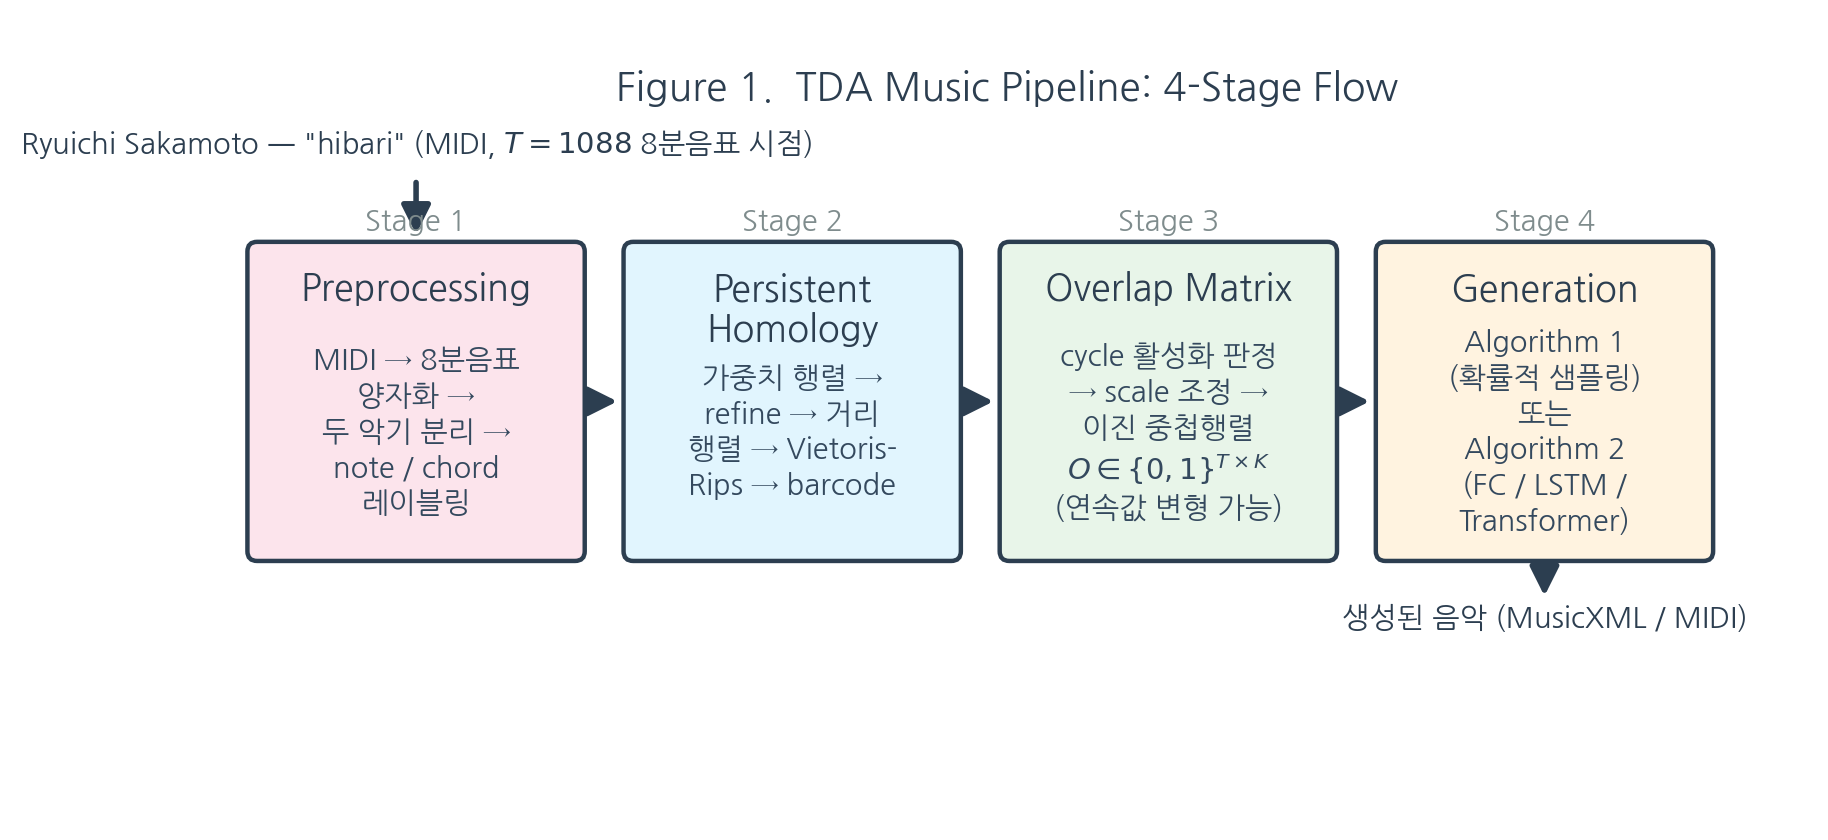
\includegraphics[width=0.96\textwidth]{fig1_pipeline.png}
\caption{Four-stage pipeline: (1)~MIDI preprocessing, (2)~persistent
homology, (3)~overlap matrix construction, (4)~generation via
Algorithm~1 or~2.}
\label{fig:pipeline}
\end{figure*}

\subsection{Stage 1: Preprocessing}
The MIDI file is quantized to 8th-note units ($T = 1{,}088$), two
instruments are separated, and each unique (pitch, duration) pair
receives a 1-indexed label ($N = 23$ notes, $C = 17$ chords for
\emph{hibari}).

\subsection{Stage 2: Persistent Homology}
A weighted note-network is constructed (\S\ref{subsec:weights}), a
distance matrix is derived, and $H_1$ filtration is computed over
$r \in [0, 1.5]$.

\subsection{Stage 3: Overlap Matrix}
Cycle activations are computed at every timepoint and thresholded
(\S\ref{subsec:overlap}).

\subsection{Algorithm 1 --- Topological Sampling}
\label{subsec:algo1}

For each timepoint~$t$:
\begin{itemize}[nosep]
\item If active cycles exist ($\sum_c O[t,c] > 0$): sample from the
      \emph{intersection} $I(t) = \bigcap_{c: O[t,c]=1} V(c)$; if
      $I(t) = \emptyset$, fall back to the union $U(t)$.
\item If no active cycle: sample from $P \setminus A(t)$, where
      $A(t) = \bigcup_{c:\, O[t-1,c]=1 \,\lor\, O[t+1,c]=1} V(c)$
      is the union of vertices belonging to cycles active at the
      immediately neighboring timepoints.  This prevents topological
      ``bleeding'' of cycle material into inactive regions.
\item Collision avoidance: up to $R = 50$ re-samples per timepoint.
\end{itemize}

\subsection{Algorithm 2 --- Neural Sequence Models}
\label{subsec:algo2}

We train three architectures on the mapping
$f_\theta : O[t,:] \mapsto y[t,:]$, where $y$ is the multi-hot note
vector:
\begin{itemize}[nosep]
\item \textbf{FC}: 2-layer fully connected ($H = 128$), timepoint-independent.
      A shallow architecture suffices because each timepoint's output
      depends only on the current overlap vector, not on temporal context.
\item \textbf{LSTM}: 2-layer, forward sequential context.
\item \textbf{Transformer}: 2-layer, 4-head, learned positional embeddings.
\end{itemize}

All models use \texttt{BCEWithLogitsLoss} with data augmentation
(subset sampling, circular shift, bit-flip noise).  At inference,
an adaptive threshold
$\theta = \mathrm{quantile}(P, 1-\rho_{\mathrm{on}})$ matches the
original ON ratio $\rho_{\mathrm{on}} = |\{(t,n): n \text{ active at } t\}| / (T \times N) \approx 0.15$,
the fraction of entries that are nonzero in the original multi-hot matrix.


% ═══════════════════════════════════════════════════════════════════════════
% SECTION 4: EXPERIMENTS
% ═══════════════════════════════════════════════════════════════════════════
\section{Experiments}
\label{sec:experiments}

All experiments use $N = 20$ independent repetitions.  The primary
metric is pitch JS divergence.

\subsection{Distance Function Comparison}
\label{subsec:dist_compare}

\begin{table}[t]
\centering
\caption{JS divergence of Algorithm~1 under four distance functions
($N = 20$, decayed lag $\ell \in \{1,\ldots,4\}$).}
\label{tab:baselines}
\begin{tabular}{lccc}
\toprule
Distance & $K$ & JS (mean $\pm$ std) & Coverage \\
\midrule
frequency      & 43 & $0.0753 \pm 0.0033$ & $0.991$ \\
\textbf{Tonnetz} & \textbf{46} & $\mathbf{0.0398 \pm 0.0031}$ & $1.000$ \\
voice-leading  & 22 & $0.0891 \pm 0.0048$ & $1.000$ \\
DFT            & 20 & $0.0511 \pm 0.0029$ & $1.000$ \\
\bottomrule
\end{tabular}
\end{table}

Tonnetz reduces JS by $47\%$ relative to frequency (Table~\ref{tab:baselines}).
Welch's $t = 35.1$, $\nu \approx 38$, $p < 10^{-20}$, Cohen's $d = 11.1$.

\subsection{Octave Weight Tuning}
\label{subsec:octave}

Grid search over $w_o \in \{0.1, 0.3, 0.5, 0.7, 1.0\}$ ($N = 10$)
found $w_o = 0.3$ optimal (JS $0.0479$, $-18.8\%$ vs.\ $w_o = 0.5$),
consistent with \emph{hibari}'s narrow 2-octave pitch range (MIDI 52--81).

\subsection{Cycle Subset Ablation}

\begin{table}[t]
\centering
\caption{Cycle subset ablation (Tonnetz, $N=20$).}
\label{tab:ablation}
\begin{tabular}{ccc}
\toprule
$K$ & JS (mean $\pm$ std) & Coverage \\
\midrule
10  & $0.0991 \pm 0.0038$ & $0.980$ \\
17  & $0.0740 \pm 0.0038$ & $0.996$ \\
46  & $\mathbf{0.0397 \pm 0.0025}$ & $1.000$ \\
\bottomrule
\end{tabular}
\end{table}

JS decreases monotonically with~$K$ (Table~\ref{tab:ablation}), but
with diminishing returns: the gain from $K{:}\,17 \to 46$ (29~extra
cycles) only marginally exceeds $K{:}\,10 \to 17$ (7~extra).

\subsection{Continuous Overlap Matrix}
\label{subsec:continuous}

\begin{table}[t]
\centering
\caption{Continuous overlap experiments (Tonnetz, $N=20$).
Density is the fraction of nonzero entries in the overlap matrix $O$.}
\label{tab:continuous}
\begin{tabular}{lcc}
\toprule
Setting & Density & JS (mean $\pm$ std) \\
\midrule
Binary (cached)           & $0.751$ & $0.0387 \pm 0.0027$ \\
Continuous direct         & $0.264$ & $0.0382 \pm 0.0021$ \\
Cont.\ $\to$ bin $\tau{=}0.3$ & $0.373$ & $0.0386 \pm 0.0022$ \\
\textbf{Cont.\ $\to$ bin $\tau{=}0.5$} & $\mathbf{0.168}$ & $\mathbf{0.0343 \pm 0.0027}$ \\
Cont.\ $\to$ bin $\tau{=}0.7$ & $0.077$ & $0.0364 \pm 0.0032$ \\
\bottomrule
\end{tabular}
\end{table}

Continuous overlap followed by $\tau = 0.5$ binarization yields an
additional $11.4\%$ improvement over the binary baseline (Welch
$t = 5.16$, $p < 0.001$, $d = 1.63$; Table~\ref{tab:continuous}).
The rarity weighting ensures rare notes contribute more to activation.

\subsection{Deep Learning Model Comparison}
\label{subsec:dl}

\begin{table}[t]
\centering
\caption{Best DL configurations (single run each).}
\label{tab:dl}
\begin{tabular}{lccc}
\toprule
Model & Val Loss & JS & Notes \\
\midrule
FC (hd=256, dropout=0.3)   & $0.282$ & $\mathbf{0.0015}$ & $3{,}754$ \\
LSTM (2-layer)         & $0.385$ & $0.0448$ & $3{,}753$ \\
Transformer (2L, 4H)   & $0.676$ & $0.0104$ & $3{,}753$ \\
\bottomrule
\end{tabular}
\end{table}

The simplest FC model achieves the lowest JS (Table~\ref{tab:dl}).
This reflects \emph{hibari}'s aesthetic: \emph{out of noise} privileges
spatial note placement over temporal causality, so a model that ignores
time context (FC) aligns better with the compositional design.

\subsection{Improvement F: Continuous Overlap + FC}
\label{subsec:improvF}

Feeding continuous activation directly to FC as training input:

\begin{table}[t]
\centering
\caption{Continuous vs.\ binary input for FC ($N=5$).}
\label{tab:improvF}
\begin{tabular}{lcccc}
\toprule
Input & JS (mean $\pm$ std) & Val Loss & Coverage \\
\midrule
Binary   & $0.0014 \pm 0.0010$ & $0.070$ & $0.948$ \\
\textbf{Continuous} & $\mathbf{0.0006 \pm 0.0005}$ & $\mathbf{0.031}$ & $\mathbf{0.991}$ \\
\bottomrule
\end{tabular}
\end{table}

Continuous input reduces JS by $57\%$ and val loss by $2.3\times$
(Table~\ref{tab:improvF}).  This is the lowest full-song JS observed
in this study ($0.09\%$ of the theoretical max $\log 2$).

\subsection{Song-Specific Structural Analysis}
\label{subsec:structure}

\paragraph{Deep scale property}
\emph{hibari}'s 7 pitch classes $\{C, D, E, F, G, A, B\}$ have interval
vector $[2,5,4,3,6,1]$---all entries distinct---a property unique to
diatonic scales \cite{gamer2003}.

\paragraph{Near-uniform pitch distribution}
\label{subsec:phase}
Normalized pitch entropy is $0.974$ (nearly maximal), explaining FC's
dominance: when all pitches are equally likely, ignoring temporal order
already approximates the true distribution.

\paragraph{Tonnetz discriminability}
With 7~PCs, the Tonnetz diameter is $4$, providing fine-grained
distance discrimination.  With all 12~PCs (as in \emph{solari}), the
diameter collapses to~$2$, erasing Tonnetz's advantage.

\paragraph{Phase shifting}
Instrument~1 repeats a 32-step module $33\times$ (no rests);
Instrument~2 repeats a 33-step module $32\times$ (one rest per module).
The coprime periods ($\gcd(32,33) = 1$) ensure the two instruments never
synchronize---a structure mathematically identical to Steve Reich's
\emph{phase shifting} technique.


% ═══════════════════════════════════════════════════════════════════════════
% SECTION 5: FIGURES
% ═══════════════════════════════════════════════════════════════════════════
\section{Figures}
\label{sec:figures}

Six static figures and one interactive HTML supplement are provided.
Fig.~\ref{fig:pipeline} shows the pipeline;
Fig.~\ref{fig:tonnetz} maps \emph{hibari}'s pitch classes on the Tonnetz
lattice; Fig.~\ref{fig:barcode} presents the persistence barcode;
Fig.~\ref{fig:pianoroll} compares original and generated piano rolls;
Fig.~\ref{fig:jscurve} plots JS vs.\ training epoch.

\begin{figure}[t]
\centering
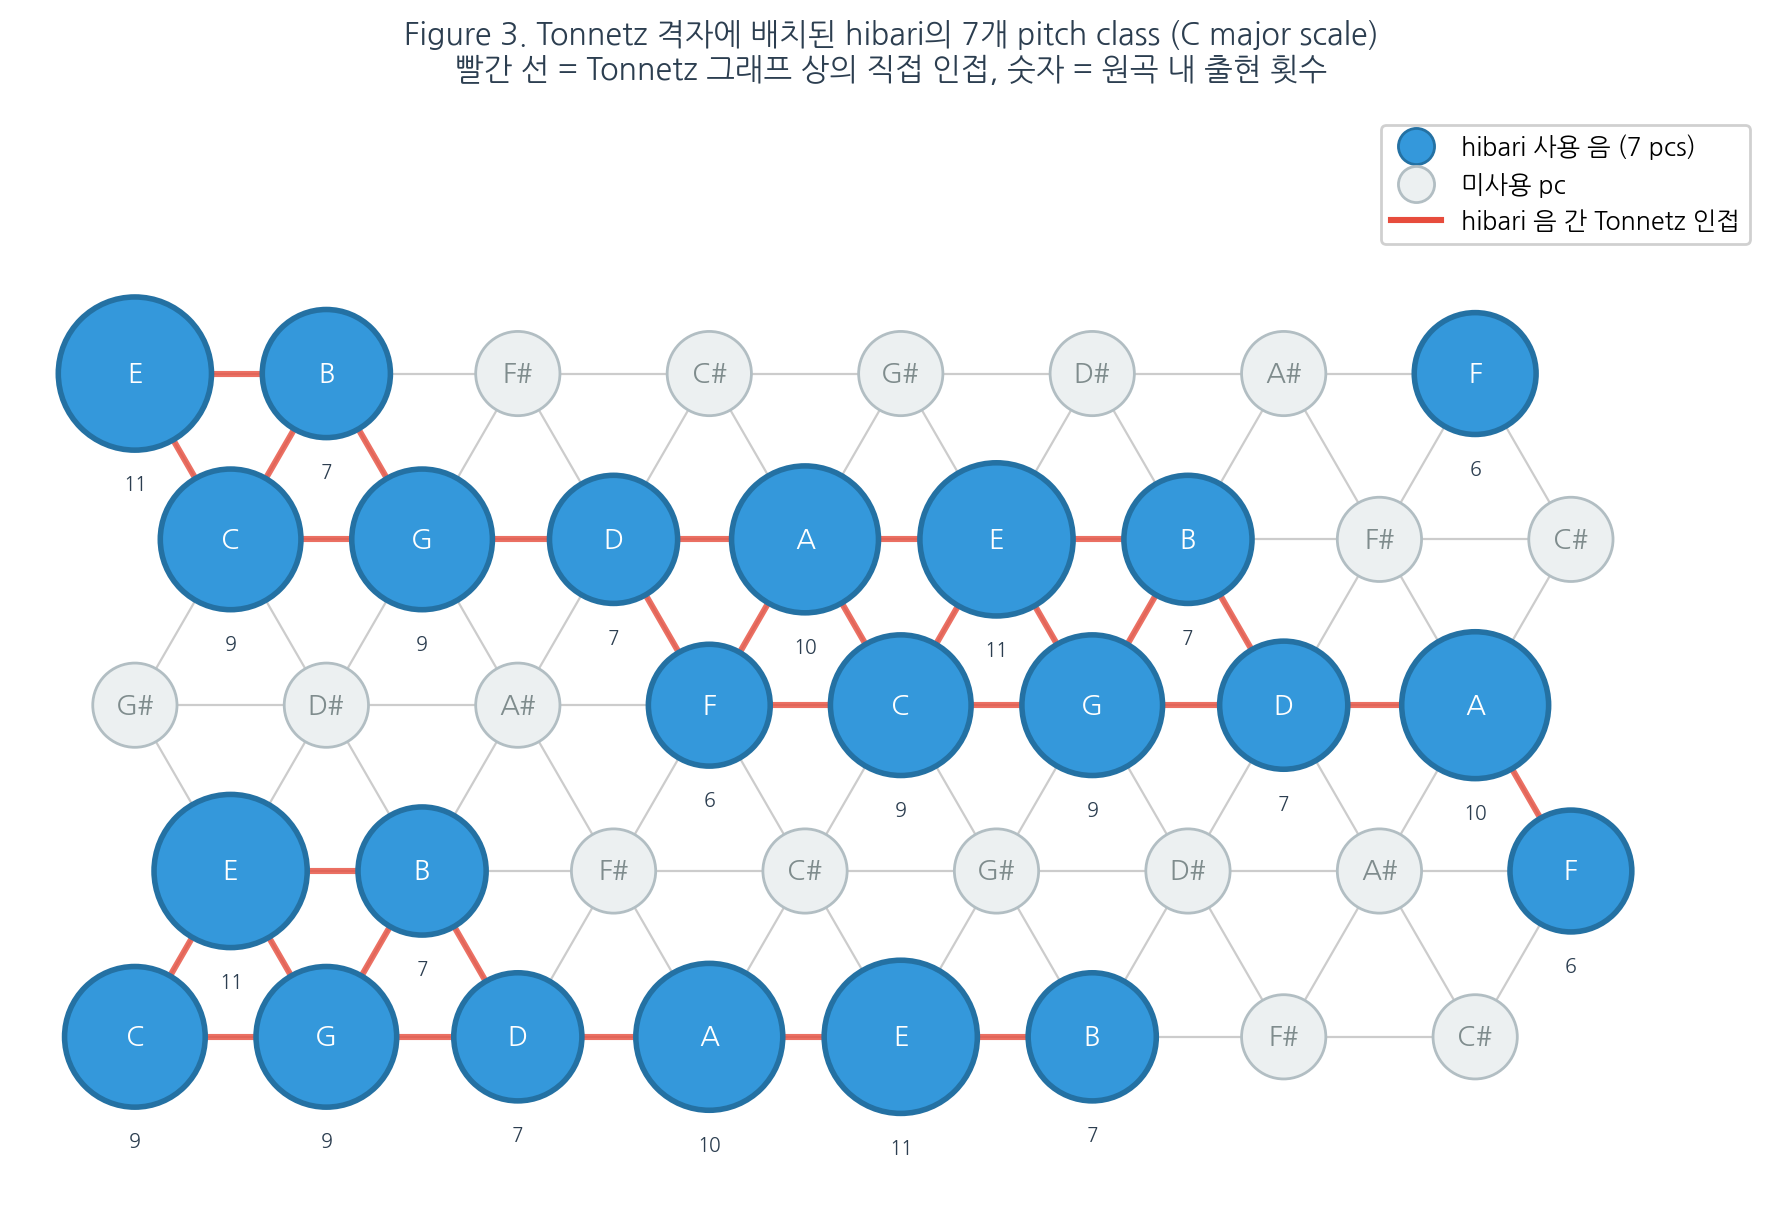
\includegraphics[width=0.99\columnwidth]{fig3_tonnetz_hibari.png}
\caption{Tonnetz lattice with \emph{hibari}'s 7 pitch classes (blue).
Red edges show direct Tonnetz adjacency.}
\label{fig:tonnetz}
\end{figure}

\begin{figure}[t]
\centering
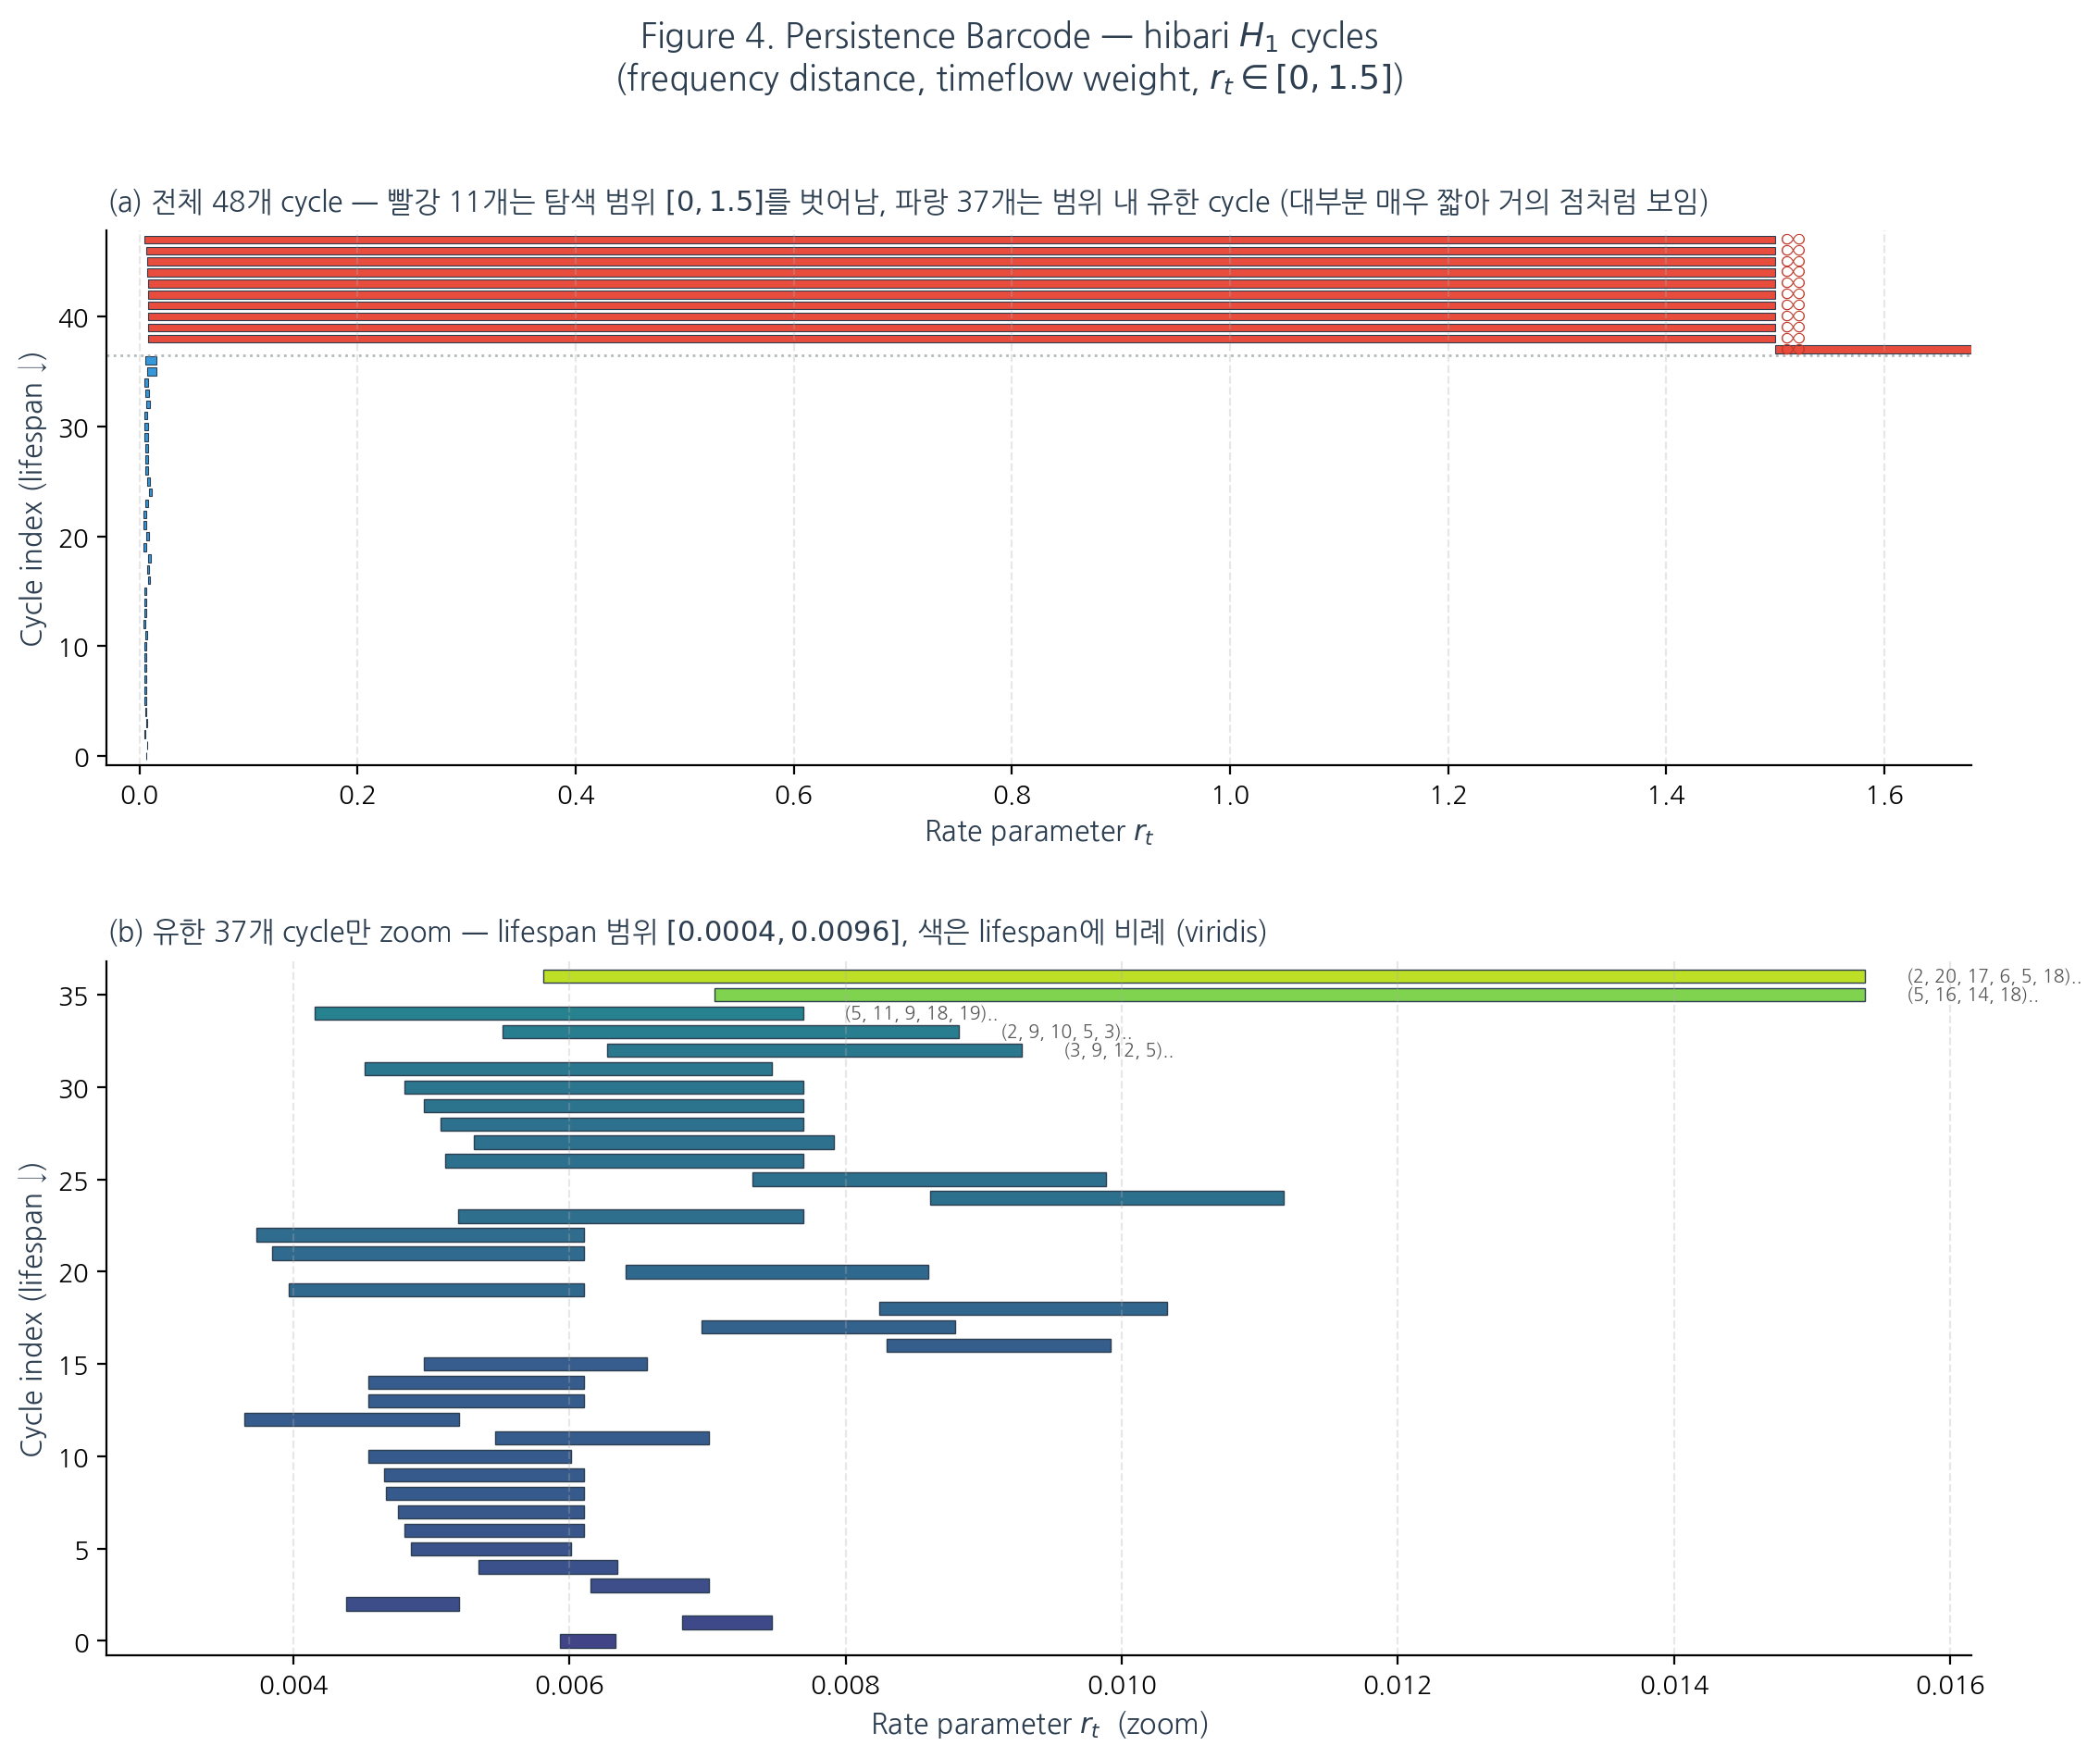
\includegraphics[width=0.99\columnwidth]{fig4_barcode.png}
\caption{$H_1$ persistence barcode (Tonnetz). Top: full barcode;
bottom: zoomed to finite cycles. Lifespan varies by $>10{,}000\times$.}
\label{fig:barcode}
\end{figure}

\begin{figure}[t]
\centering
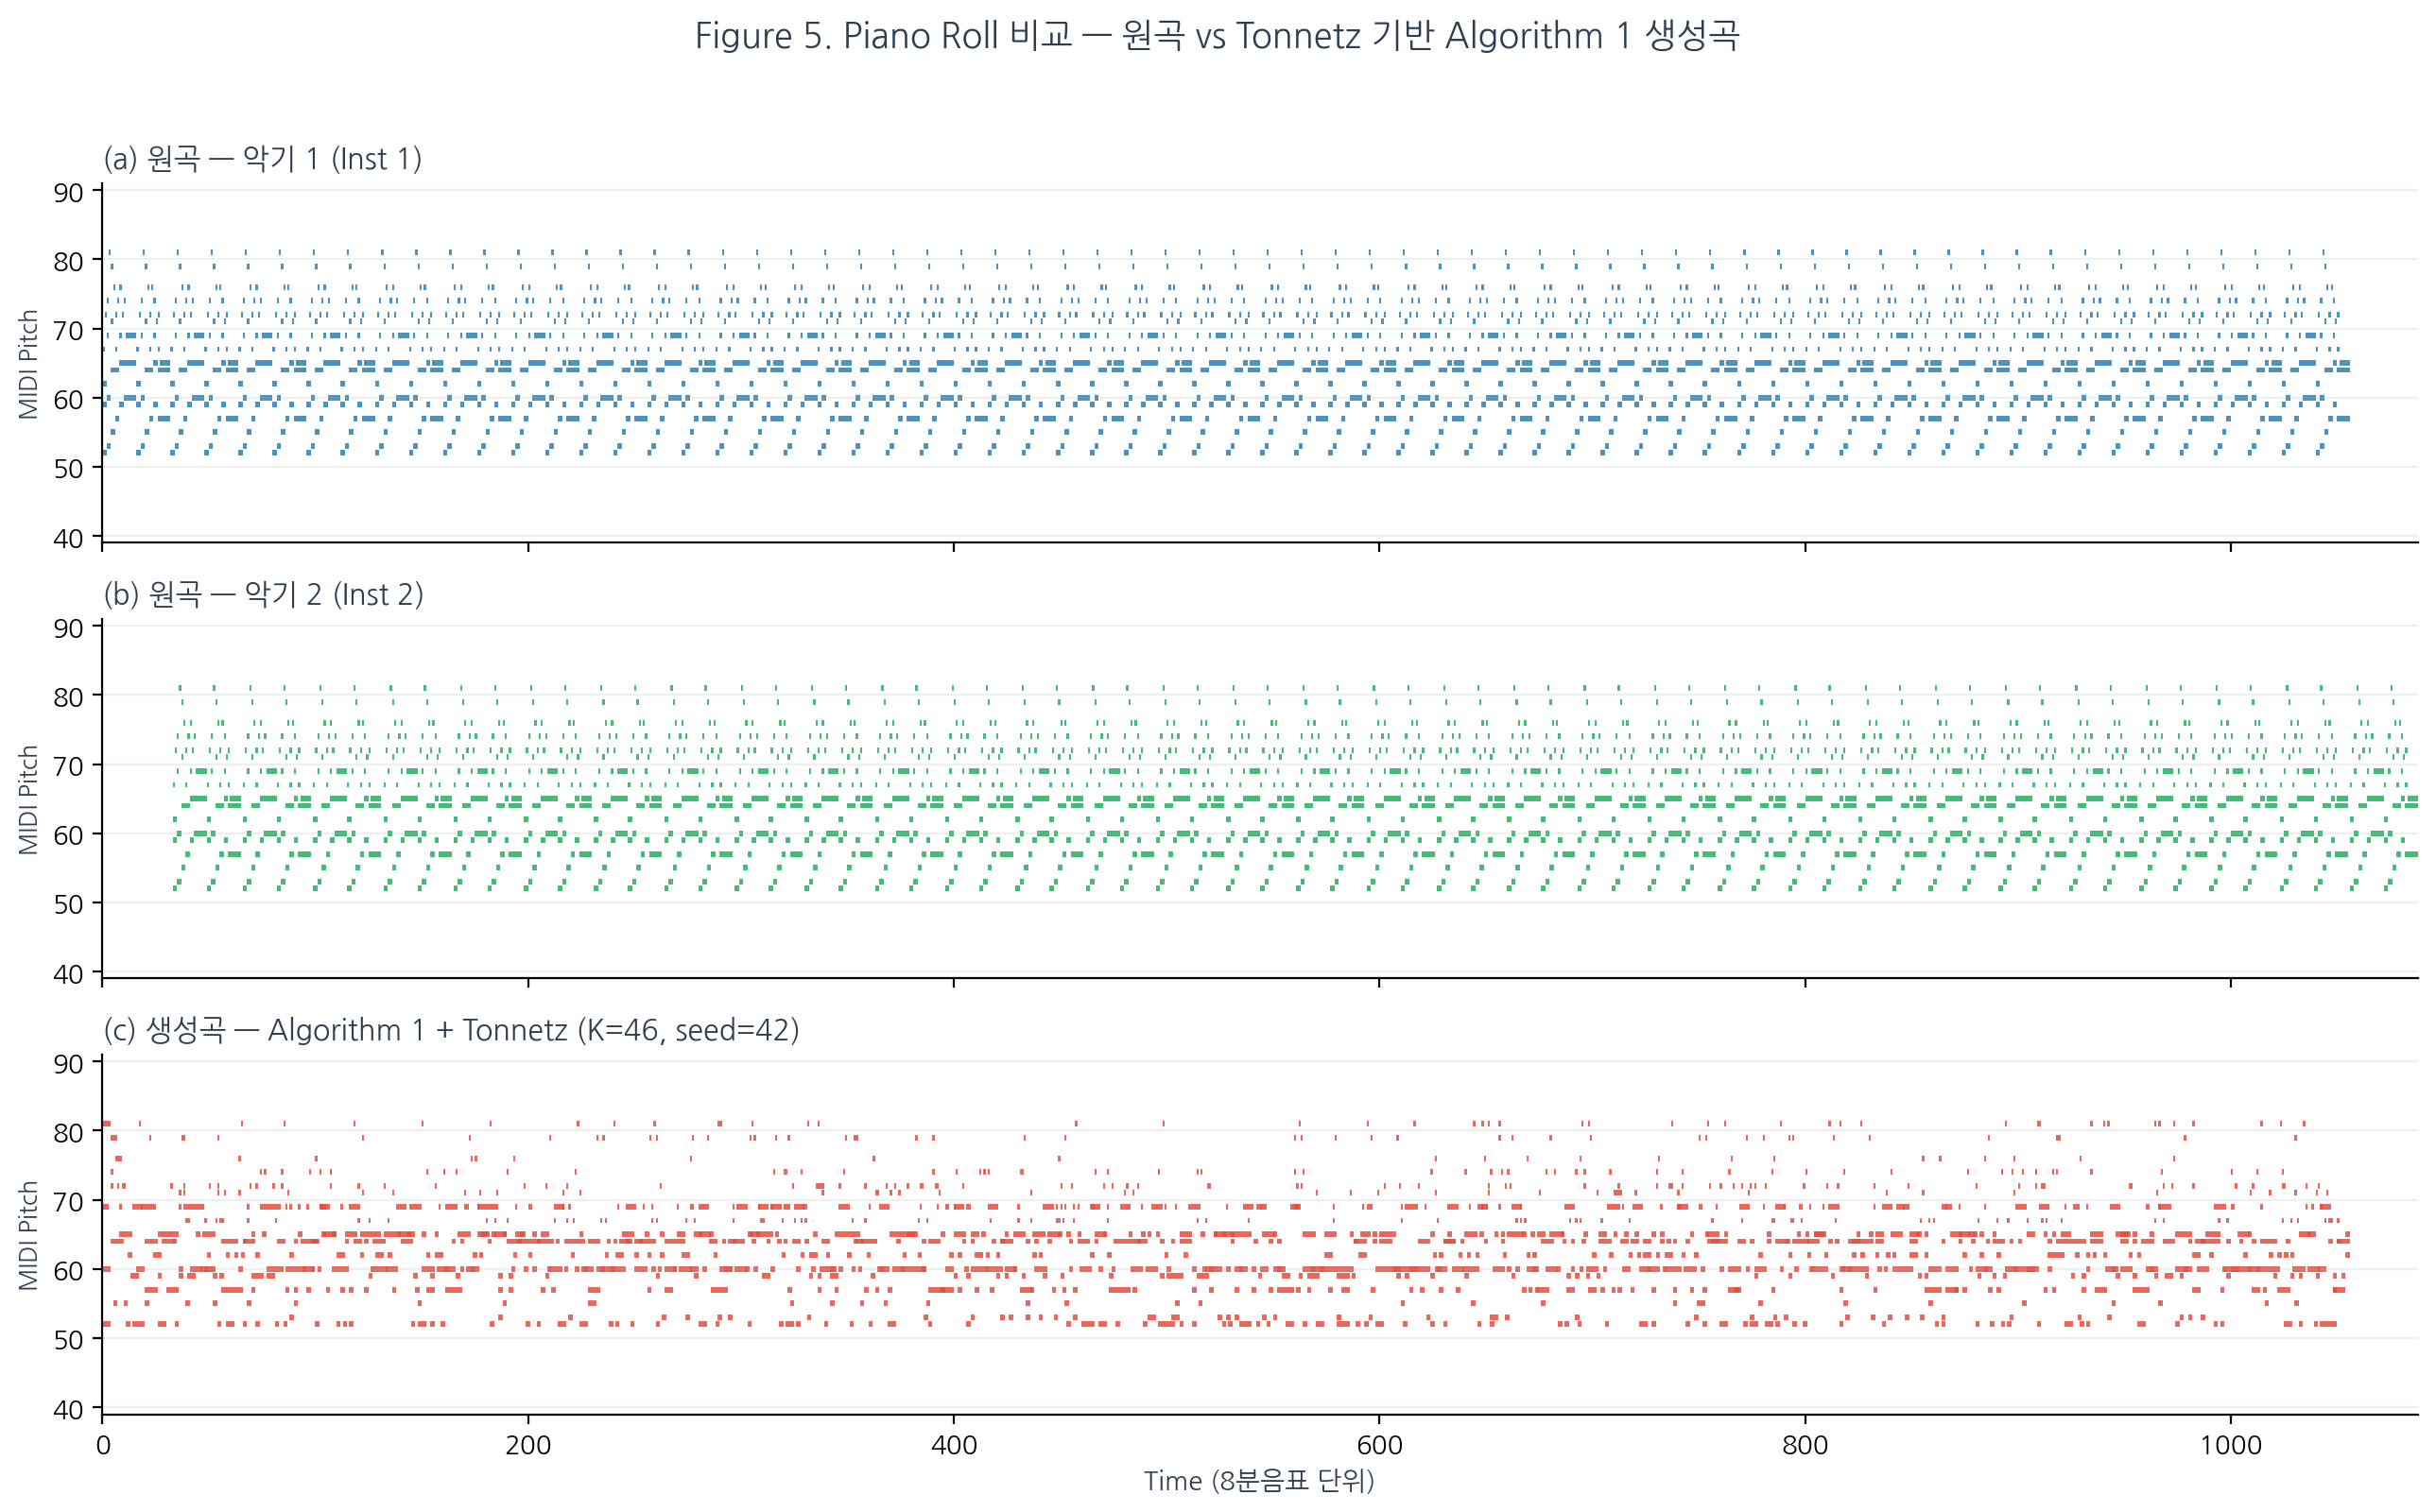
\includegraphics[width=0.99\columnwidth]{fig5_pianoroll.png}
\caption{Piano roll comparison: (a)--(b) original instruments 1--2;
(c)~Algorithm~1 + Tonnetz.}
\label{fig:pianoroll}
\end{figure}

\begin{figure}[t]
\centering
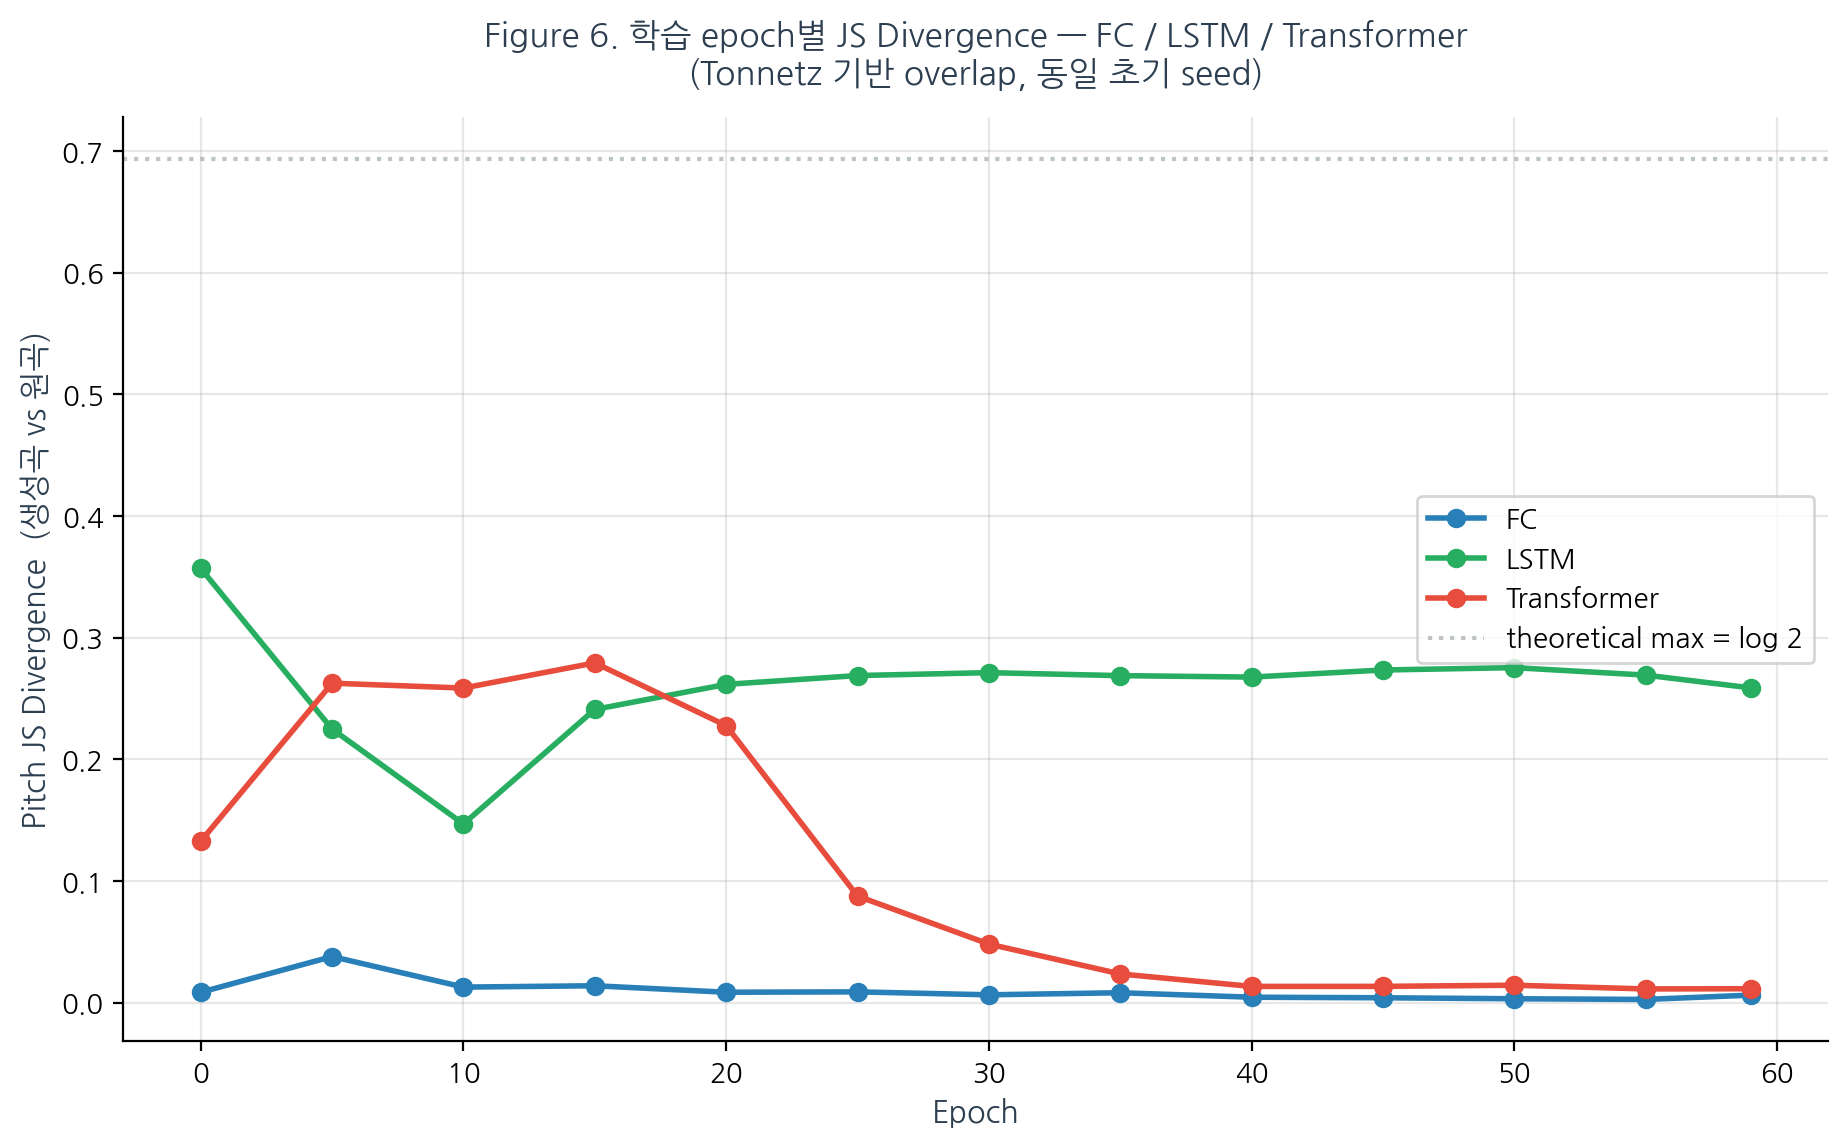
\includegraphics[width=0.99\columnwidth]{fig6_js_curve.png}
\caption{JS divergence vs.\ training epoch. FC converges fastest;
LSTM plateaus at $\mathrm{JS} \approx 0.26$.}
\label{fig:jscurve}
\end{figure}


% ═══════════════════════════════════════════════════════════════════════════
% SECTION 6: DIFFERENTIATION
% ═══════════════════════════════════════════════════════════════════════════
\section{Comparison with Related Work}
\label{sec:differentiation}

\subsection{vs.\ General AI Music Generation}

Unlike corpus-trained models (Magenta, Music Transformer), our pipeline
performs \emph{deep analysis of a single composition}, yielding
interpretable, traceable generation.  The FC~$>$~Transformer finding
challenges the universal assumption that more temporal modeling is better.

\subsection{vs.\ Existing TDA--Music Research}

Compared to prior TDA--music work \cite{tran2021,lee2024}:
(A)~we systematically compare four distance functions with $N{=}20$
    statistics;
(B)~we introduce continuous overlap matrices;
(C)~we provide full statistical rigor (Welch $t$, Cohen's $d$);
(D)~we extend to Western contemporary music;
(E)~we connect model selection to aesthetic context;
(F)~we extend TDA from analysis to \emph{variation} (\S\ref{sec:extensions}).


% ═══════════════════════════════════════════════════════════════════════════
% SECTION 7: EXTENSION EXPERIMENTS
% ═══════════════════════════════════════════════════════════════════════════
\section{Extension Experiments}
\label{sec:extensions}

\subsection{Module-Level Generation}
\label{subsec:module}

\emph{hibari}'s 32-step modular structure motivates generating a single
module and replicating it $33\times$.  Five prototype strategies for
constructing a 32-step module overlap vector were compared:
\begin{itemize}[nosep]
\item \textbf{P0}: element-wise OR of all module instances (any-active).
\item \textbf{P1}: element-wise mean across modules, binarized at $\tau{=}0.5$.
\item \textbf{P2}: element-wise mean without binarization (continuous prototype).
\item \textbf{P3}: element-wise median across modules.
\item \textbf{P5}: flat control (all entries set to the global mean).
\end{itemize}
P4 takes a different approach: instead of aggregating the full-song
overlap matrix, it runs module-local persistent homology on the first
module alone ($K{=}24$ cycles).  P4 combined with best-of-10
selection~(C) achieved the best result:

\begin{table}[t]
\centering
\caption{Module-level generation strategies ($N=10$).}
\label{tab:module}
\begin{tabular}{lcccc}
\toprule
Strategy & JS (mean$\pm$std) & Best & Cov. \\
\midrule
P1 baseline      & $0.114 \pm 0.039$ & $0.074$ & $0.77$ \\
C: best-of-10    & $0.074 \pm 0.027$ & $0.024$ & $0.90$ \\
D: cov$\ge$20/23 & $0.082 \pm 0.022$ & $0.050$ & $0.88$ \\
P4: local PH     & $0.066 \pm 0.019$ & $0.038$ & $0.84$ \\
\textbf{P4+C}    & $\mathbf{0.059 \pm 0.015}$ & $\mathbf{0.026}$ & $0.89$ \\
\bottomrule
\end{tabular}
\end{table}

Start-module analysis over 8 positions confirmed module~0
($t \in [0,32)$) as optimal (JS~$0.054$, best~$0.026$), consistent with
minimalist composition practice of presenting core material in the
opening module.  The best single trial (seed~9302, JS~$= 0.0258$)
outperforms the full-song baseline mean ($0.0398$).

\subsection{Generalization: \emph{solari}, Bach, Ravel}
\label{subsec:generalization}

\begin{table}[t]
\centering
\caption{Cross-composition summary.  ``---'' indicates that Algorithm~2
(deep learning) was not tested for that piece; only Algorithm~1 results
are reported.}
\label{tab:generalization}
\begin{tabular}{lcccc}
\toprule
Piece & PCs & Best dist. & Best model & Interpretation \\
\midrule
hibari & 7 & Tonnetz & FC & Spatial placement \\
solari & 12 & freq/Ton. & Transformer & Melodic progression \\
aqua   & 12 & Tonnetz & --- & Tonnetz $+26.3\%$ \\
Bach   & 12 & Tonnetz & --- & Tonnetz $-54.8\%$ \\
Ravel  & 12 & frequency & FC & Rich distribution \\
\bottomrule
\end{tabular}
\end{table}

On \emph{solari} (12-PC, chromatic), Transformer is optimal
(JS~$0.016$), exactly reversing \emph{hibari}'s FC dominance
(Table~\ref{tab:generalization}).  On Bach Fugue, Tonnetz achieves
$-54.8\%$, the largest improvement observed.  On Ravel Pavane ($N{=}49$
notes), frequency is optimal, suggesting that rich note diversity favors
frequency-based separation.

\subsection{Direction A: Two-Strategy Note Redistribution}
\label{subsec:dirA}

The overlap matrix is preserved intact; only note identities change.
We compare two exclusive matching strategies over $n_{\mathrm{cand}}=1000$
candidate pitch sets ($N=20$ trials, \emph{hibari}, Tonnetz, MIDI~48--84).

\textbf{Strategy A --- Positional Tonnetz nearest-neighbour
(\texttt{tonnetz\_nearest}):}
\begin{equation}
\mathrm{new\_pitches}[i]
  = \arg\min_{p\,\in\,\mathrm{pool}}\,d_{\mathrm{Tonnetz}}
    \!\bigl(\mathrm{orig\_pitches}[i],\,p\bigr).
\end{equation}
Each original note is replaced by its closest pool element in Tonnetz
space; the index~$i$ encodes a 1:1 positional correspondence that
preserves local harmonic relations.

\textbf{Strategy B --- Matrix-structure Hungarian matching
(\texttt{ascending}):}
\begin{equation}
\pi^{*} = \arg\min_{\pi}\,
  \bigl\|P_{\pi}\,\hat{D}_{\mathrm{new}}\,P_{\pi}^{\top}
         - \hat{D}_{\mathrm{orig}}\bigr\|_{F},
\end{equation}
where $\hat{D}$ is the off-diagonal min-max normalised distance matrix:
\begin{equation}
\hat{D}_{ij}
  = \frac{D_{ij}-\min_{k\neq l}D_{kl}}
         {\max D - \min_{k\neq l}D_{kl}},
\quad \hat{D}_{ii}=0.
\end{equation}
Solving the joint row-column permutation exactly is NP-hard; with
$N=17$ notes, $N!\!=3.56\times10^{14}$ exhaustive evaluations are
infeasible, so all experiments use the Hungarian approximation
(\texttt{scipy.optimize.linear\_sum\_assignment}).

Both strategies report \textbf{note\_dist\_error}
$=\|\hat{D}_{\mathrm{orig}}-\hat{D}_{\mathrm{new}}\|_F$,
which is on the same $\hat{D}$ scale and directly comparable across rows.
Applying both strategies simultaneously degrades performance (Strategy~A's
positional semantics are overwritten by Strategy~B's permutation), so the
two are applied exclusively via \texttt{matching\_mode}.

\begin{table}[t]
\centering
\caption{Two-strategy comparison (Algorithm~1, Tonnetz, MIDI~48--84,
         $N=20$, $n_{\mathrm{cand}}=1000$).}
\label{tab:redistrib}
\begin{tabular}{lcccc}
\toprule
Strategy & pitch JS & trans.\ JS & DTW & note err \\
\midrule
baseline (original)
  & $0.0212$ & $0.2470$ & $2.2186$ & --- \\
B: ascending (Hungarian)
  & $0.3815$ & $0.6121$ & $2.7918$ & $4.6819$ \\
\textbf{A: \texttt{tonnetz\_nearest}}
  & $\mathbf{0.2930}$ & $\mathbf{0.5488}$ & $2.6442$ & $\mathbf{3.2132}$ \\
\bottomrule
\end{tabular}
\end{table}

Strategy~A achieves pitch~JS $0.2930$ vs.\ $0.3815$ for Strategy~B
($-23.2\%$, Table~\ref{tab:redistrib}).  Local pairwise harmonic
preservation~(A) outperforms global distance-matrix alignment~(B),
consistent with \emph{hibari}'s small note vocabulary ($N=17$) in which
adjacent Tonnetz relations directly govern harmonic character
(\S\ref{subsec:structure}).  The wider pitch range vwide (MIDI~40--88)
was inferior to wide (48--84) in all conditions; wide is adopted.

\subsection{Direction B: Temporal Reordering}
\label{subsec:dirB}

Two strategies were tested: block permutation (dividing the sequence
into fixed-size blocks and randomly permuting them; also called
``segment shuffle'' in our codebase) and Markov resampling.
With PE removal and retraining, Transformer
achieves DTW~$+21.7\%$, but pitch JS degrades from $0.007$ to $0.173$.
Direction~B alone cannot simultaneously preserve pitch distribution and
alter melody; it requires combination with Direction~A.

\subsection{Harmonic Constraints}
\label{subsec:harmony}

Scale constraints (major, minor, pentatonic) and consonance objectives
were added to note redistribution.  \textbf{scale\_major} was most
effective: note error $4.35 \to 3.52$ ($-19\%$), scale match $1.00$,
average dissonance $0.412 \to 0.361$.

\subsection{Combined A+B: Final Integration}
\label{subsec:combined}

The best combined setting (\textbf{major\_block32}):
scale\_major redistribution + block permutation(32) + continuous
overlap + Transformer achieves:
ref~pJS $= 0.002$ (near-perfect learning),
DTW $+31\%$ (different melody),
C~major scale match $= 1.00$.

\subsection{Per-Cycle Threshold Optimization}
\label{subsec:percycle}

Greedy coordinate descent over
$\tau_c \in \{0.1, 0.2, \ldots, 0.7\}$ for each cycle:

\begin{table}[t]
\centering
\caption{Per-cycle $\tau_c$ optimization ($N=20$).}
\label{tab:percycle}
\begin{tabular}{lcc}
\toprule
Setting & JS (mean $\pm$ std) & Improvement \\
\midrule
Uniform $\tau = 0.35$ & $0.0460 \pm 0.0034$ & --- \\
\textbf{Per-cycle $\tau_c$} & $\mathbf{0.0241 \pm 0.0023}$ & $\mathbf{+47.5\%}$ \\
\bottomrule
\end{tabular}
\end{table}

$47.5\%$ improvement ($p < 0.001$; Table~\ref{tab:percycle}).  The
majority of cycles prefer $\tau < 0.35$, suggesting that ``accompaniment-type'' cycles were
previously suppressed.  No overfitting: N=5 greedy result ($0.0238$) matches N=20 ($0.0241$).

\subsection{Soft Activation: All Architectures}
\label{subsec:soft}

\begin{table}[t]
\centering
\caption{Binary vs.\ continuous input ($N=5$).}
\label{tab:soft}
\begin{tabular}{llccc}
\toprule
Model & Input & JS & Val Loss & $\Delta$JS \\
\midrule
FC   & Binary & $0.0035$ & $0.307$ & --- \\
\textbf{FC} & \textbf{Cont.} & $\mathbf{0.0004}$ & $\mathbf{0.026}$ & $\mathbf{+88.6\%}$ \\
Trans. & Binary & $0.0034$ & $0.465$ & --- \\
\textbf{Trans.} & \textbf{Cont.} & $\mathbf{0.0007}$ & $\mathbf{0.121}$ & $\mathbf{+79.4\%}$ \\
LSTM & Binary & $0.280$ & $0.411$ & --- \\
LSTM & Cont. & $0.290$ & $0.411$ & $-3.5\%$ \\
\bottomrule
\end{tabular}
\end{table}

FC and Transformer show massive improvement with continuous input;
LSTM is incompatible (Table~\ref{tab:soft}).  FC + continuous
achieves JS~$= 0.0004$---the overall best in this study.

\subsection{Tonnetz $\alpha$ Grid Search}
\label{subsec:alpha}

\begin{table}[t]
\centering
\caption{$\alpha$ grid search ($N=20$).}
\label{tab:alpha}
\begin{tabular}{cccc}
\toprule
$\alpha$ & $K$ & JS (mean $\pm$ std) & Note \\
\midrule
$0.0$ & 14 & $\mathbf{0.0574 \pm 0.0023}$ & Best among $K \ge 14$ \\
$0.3$ & 48 & $0.0870 \pm 0.0046$ & Worst \\
$0.5$ & 42 & $0.0594 \pm 0.0033$ & Default \\
$1.0$ & 1  & $0.0351 \pm 0.0020$ & Degenerate ($K{=}1$) \\
\bottomrule
\end{tabular}
\end{table}

$\alpha = 0.0$ (pure Tonnetz) is individually optimal, but combined
with $w_o = 0.3$ and decayed lag, cycle count collapses to $K = 14$.
To maintain topological diversity ($K = 42$), we retain
$\alpha = 0.5$ as the default (Table~\ref{tab:alpha}).

\subsection{Barcode Wasserstein Module Selection}
\label{subsec:wasserstein}

For each candidate start module at position~$m$, we compute the
persistence diagram $\mathrm{PD}_m$ from the module-local chord
sequence (32~timepoints, single instrument) and compare it to the
full-song persistence diagram~$\mathrm{PD}_{\mathrm{full}}$ via the
Wasserstein distance $W_1(\mathrm{PD}_m, \mathrm{PD}_{\mathrm{full}})$.
The hypothesis is that modules whose local topology most closely
resembles the global topology will yield lower generation JS.

Across 8~start positions, the Pearson correlation between $W_1$ and
generation JS is $r = 0.503$---moderate but not decisive.  Three
caveats limit its applicability:
\begin{enumerate}[nosep]
\item \textbf{Chord-space mismatch}: module-local PD is computed from
      a 32-step window, whose chord vocabulary is a strict subset of
      the full song's.  The resulting PD inhabits a smaller simplicial
      complex.
\item \textbf{Single-instrument limitation}: module-local PH uses only
      one instrument's note sequence, so inter-instrument weight
      information (which contributes the largest JS gains via decayed
      lag weighting) is entirely absent.
\item \textbf{Scale sensitivity}: $W_1$ is sensitive to the absolute
      scale of birth/death coordinates, which differ between a 32-step
      and a 1{,}088-step filtration.
\end{enumerate}
We therefore position Wasserstein module selection as a supplementary
tiebreaker rather than a primary selection criterion.

% ═══════════════════════════════════════════════════════════════════════════
% SECTION 8: CONCLUSION
% ═══════════════════════════════════════════════════════════════════════════
\section{Conclusion}
\label{sec:conclusion}

We presented a unified pipeline that extracts topological structure from
music via persistent homology and generates new music preserving that
structure.  Key findings:

\begin{enumerate}
\item \textbf{Distance function matters.} Tonnetz reduces JS by $47\%$
      on \emph{hibari} ($p < 10^{-20}$), but this advantage is
      composition-specific: Bach Fugue shows $-54.8\%$ Tonnetz
      improvement, while Ravel Pavane favors frequency.

\item \textbf{Composition character determines optimal model.}
      \emph{hibari} (diatonic, entropy $0.974$) $\to$ FC;
      \emph{solari} (chromatic, entropy $0.905$) $\to$ Transformer.

\item \textbf{Continuous overlap is powerful.} Per-cycle thresholding
      adds $47.5\%$ ($p < 0.001$); soft activation input yields
      $+88.6\%$ (FC) and $+79.4\%$ (Transformer).

\item \textbf{Topology-preserving variation is feasible.} Note
      redistribution + temporal reordering + harmonic constraints
      produce music with DTW $+31\%$ (different melody), ref pJS $0.002$
      (accurate learning), and perfect C major scale match.

\item \textbf{Module-level generation is competitive.} P4+C achieves
      JS~$0.059$ (average) with best trial $0.026$ outperforming the
      full-song baseline---extending the pipeline to real-time
      interactive composition tools.
\end{enumerate}

This work demonstrates that TDA can serve not only as an analysis tool
but as a \emph{constraint generator for musical creation}, bridging
mathematical topology and compositional aesthetics.


% ═══════════════════════════════════════════════════════════════════════════
% ACKNOWLEDGMENTS
% ═══════════════════════════════════════════════════════════════════════════
\section*{Acknowledgments}

This research was conducted under the guidance of Prof.~Jae-Hun Jung.
We acknowledge
the foundational pHcol implementation and pipeline design inherited from
the preceding study on Korean traditional music \cite{lee2024}.


% ═══════════════════════════════════════════════════════════════════════════
% BIBLIOGRAPHY
% ═══════════════════════════════════════════════════════════════════════════
\begin{thebibliography}{99}

\bibitem{carlsson2009}
G.~Carlsson, ``Topology and data,''
\emph{Bulletin of the AMS}, vol.~46, no.~2, pp.~255--308, 2009.

\bibitem{edelsbrunner2010}
H.~Edelsbrunner and J.~Harer,
\emph{Computational Topology: An Introduction}. AMS, 2010.

\bibitem{tymoczko2012}
D.~Tymoczko, ``The generalized Tonnetz,''
\emph{J.\ Music Theory}, vol.~56, no.~1, 2012.

\bibitem{tymoczko2008}
D.~Tymoczko, ``Set-class similarity, voice leading, and the Fourier
transform,'' \emph{J.\ Music Theory}, vol.~52, no.~2, 2008.

\bibitem{bauer2021}
U.~Bauer, ``Ripser: Efficient computation of Vietoris--Rips persistence
barcodes,'' \emph{J.\ Applied and Computational Topology}, vol.~5,
pp.~391--423, 2021.

\bibitem{tran2021}
M.~L.~Tran, C.~Park, and J.-H.~Jung, ``Topological data analysis of
Korean music in Jeongganbo,'' \emph{arXiv:2103.06620}, 2021.

\bibitem{lee2024}
D.-J.~Lee, M.~L.~Tran, and J.-H.~Jung, ``Geometric structure and AI
composition of Korean traditional music,'' 2024.

\bibitem{heo2025}
E.~Heo, B.~Choi, and J.-H.~Jung, ``Persistent homology with
path-representable distances on graph data,''
\emph{arXiv:2501.03553}, 2025.

\bibitem{nemhauser1978}
G.~L.~Nemhauser, L.~A.~Wolsey, and M.~L.~Fisher, ``An analysis of
approximations for maximizing submodular set functions,''
\emph{Math.\ Programming}, vol.~14, no.~1, pp.~265--294, 1978.

\bibitem{welch1947}
B.~L.~Welch, ``The generalization of `Student's' problem when several
different population variances are involved,''
\emph{Biometrika}, vol.~34, pp.~28--35, 1947.

\bibitem{cohen1988}
J.~Cohen, \emph{Statistical Power Analysis for the Behavioral Sciences},
2nd~ed. Lawrence Erlbaum, 1988.

\bibitem{hochreiter1997}
S.~Hochreiter and J.~Schmidhuber, ``Long short-term memory,''
\emph{Neural Computation}, vol.~9, no.~8, pp.~1735--1780, 1997.

\bibitem{vaswani2017}
A.~Vaswani \emph{et al.}, ``Attention is all you need,'' in
\emph{Proc.\ NeurIPS}, 2017.

\bibitem{sakamoto2009}
R.~Sakamoto, \emph{out of noise} [Album]. commmons, 2009.

\bibitem{gamer2003}
C.~Gamer and R.~Wilson, ``Microtones and projective planes,'' in
\emph{Music and Mathematics}. Oxford University Press, 2003.

\end{thebibliography}

\end{document}
